\documentclass[letterpaper,12pt]{article}
\usepackage[left=3cm,right=2cm,top=3.5cm,bottom=2.5cm,headheight=15pt]{geometry}
\usepackage[T1]{fontenc}
\usepackage[utf8]{inputenc}
\usepackage[spanish,es-tabla]{babel}
\usepackage{graphicx,tabularx,array,float,xcolor,listings,fancyhdr,lastpage}
\usepackage[hidelinks]{hyperref}
\graphicspath{{imagenes/}}
\pagestyle{fancy}
\fancyhf{}
\fancyhead[L]{\small Laboratorio 2}
\fancyhead[R]{\small Pablo Muñoz R}
\fancyfoot[C]{\thepage}
\setlength{\emergencystretch}{3em}
\lstset{basicstyle=\ttfamily\footnotesize,breaklines=true,columns=fullflexible,keepspaces=true,showstringspaces=false,frame=single}
\newcommand{\evidencia}[3]{\begin{figure}[H]\centering\includegraphics[width=\linewidth,height=.60\textheight,keepaspectratio]{#1}\caption{#2}\label{#3}\end{figure}}
\newcommand{\pendiente}[1]{\par\noindent\fbox{\parbox{.94\linewidth}{\textbf{Evidencia pendiente:} #1}}\par}
\begin{document}
\title{\Huge Informe Laboratorio 2}
\author{\textbf{Sección 4}\\Pablo Muñoz R\\\texttt{pablo.munoz5@mail.udp.cl}}
\date{Octubre de 2026}
\maketitle
\tableofcontents
\newpage
\section{Descripción de actividades}
En este laboratorio se utilizó la aplicación web vulnerable DVWA (Damn Vulnerable Web Application), disponible en \url{https://github.com/digininja/DVWA}. El trabajo se desarrolló localmente en macOS, utilizando Docker para ejecutar la aplicación y su base de datos. Las pruebas se realizaron sobre el formulario \texttt{vulnerabilities/brute}, configurando el nivel de seguridad en \texttt{low}.
\begin{itemize}
\item Desplegar DVWA mediante Docker y explicar la redirección de puertos utilizada.
\item Utilizar Burp Suite para capturar una petición y realizar un ataque de diccionario, obteniendo al menos dos pares válidos.
\item Copiar una petición desde las herramientas del navegador y ejecutarla con cURL, comparando un acceso válido con uno inválido.
\item Utilizar Hydra para automatizar los intentos y obtener al menos dos pares válidos.
\item Capturar el tráfico con Wireshark y comparar los mensajes generados por las tres herramientas.
\end{itemize}
\section{Desarrollo de actividades según criterio de rúbrica}
\subsection{Levantamiento de Docker para correr DVWA (dvwa)}
Para esta actividad se utilizó Docker Desktop, previamente instalado en el equipo. Luego de clonar el repositorio de DVWA, se ingresó a la carpeta del proyecto y se levantaron los servicios definidos en el archivo \texttt{compose.yml}:
\begin{lstlisting}
cd /Users/pablo/Desktop/lab2_cripto/DVWA
docker compose up -d
docker compose ps
\end{lstlisting}
El comando \texttt{up} crea e inicia los servicios, mientras que \texttt{-d} permite mantenerlos ejecutándose en segundo plano. El archivo Compose define un servicio para DVWA y otro para MariaDB. La base de datos utiliza un volumen para conservar sus datos entre reinicios de los contenedores.
Una vez iniciados los servicios, se accedió a \url{http://127.0.0.1:4280/setup.php} y se utilizó la opción \textit{Create / Reset Database}. Posteriormente se inició sesión con el usuario \texttt{admin} y la contraseña \texttt{password}, y se seleccionó el nivel \texttt{Low} en DVWA Security.
En la Figura~\ref{fig:dockerestado} se observa la ejecución de los comandos y ambos servicios en funcionamiento. La salida corresponde a una comprobación posterior del entorno, ya que los contenedores se encontraban creados previamente.
\evidencia{docker_estado.jpg}{Ejecución de Docker Compose y comprobación de los servicios DVWA y MariaDB.}{fig:dockerestado}
\subsection{Redirección de puertos en Docker (dvwa)}
La configuración del servicio DVWA contiene la siguiente publicación de puertos:
\begin{lstlisting}
ports:
  - 127.0.0.1:4280:80
\end{lstlisting}
La dirección \texttt{127.0.0.1} limita el acceso al equipo local. El puerto \texttt{4280} corresponde al puerto utilizado en el Mac, mientras que \texttt{80} corresponde al servidor web dentro del contenedor. De esta forma, al ingresar a \url{http://127.0.0.1:4280}, Docker dirige la conexión hacia DVWA.
La Figura~\ref{fig:dockercompose} muestra la configuración utilizada. Además, la columna PORTS de la Figura~\ref{fig:dockerestado} confirma la publicación efectiva de \texttt{127.0.0.1:4280->80/tcp}. MariaDB muestra \texttt{3306/tcp} sin un puerto publicado en el equipo anfitrión.
\begin{figure}[p]
\centering
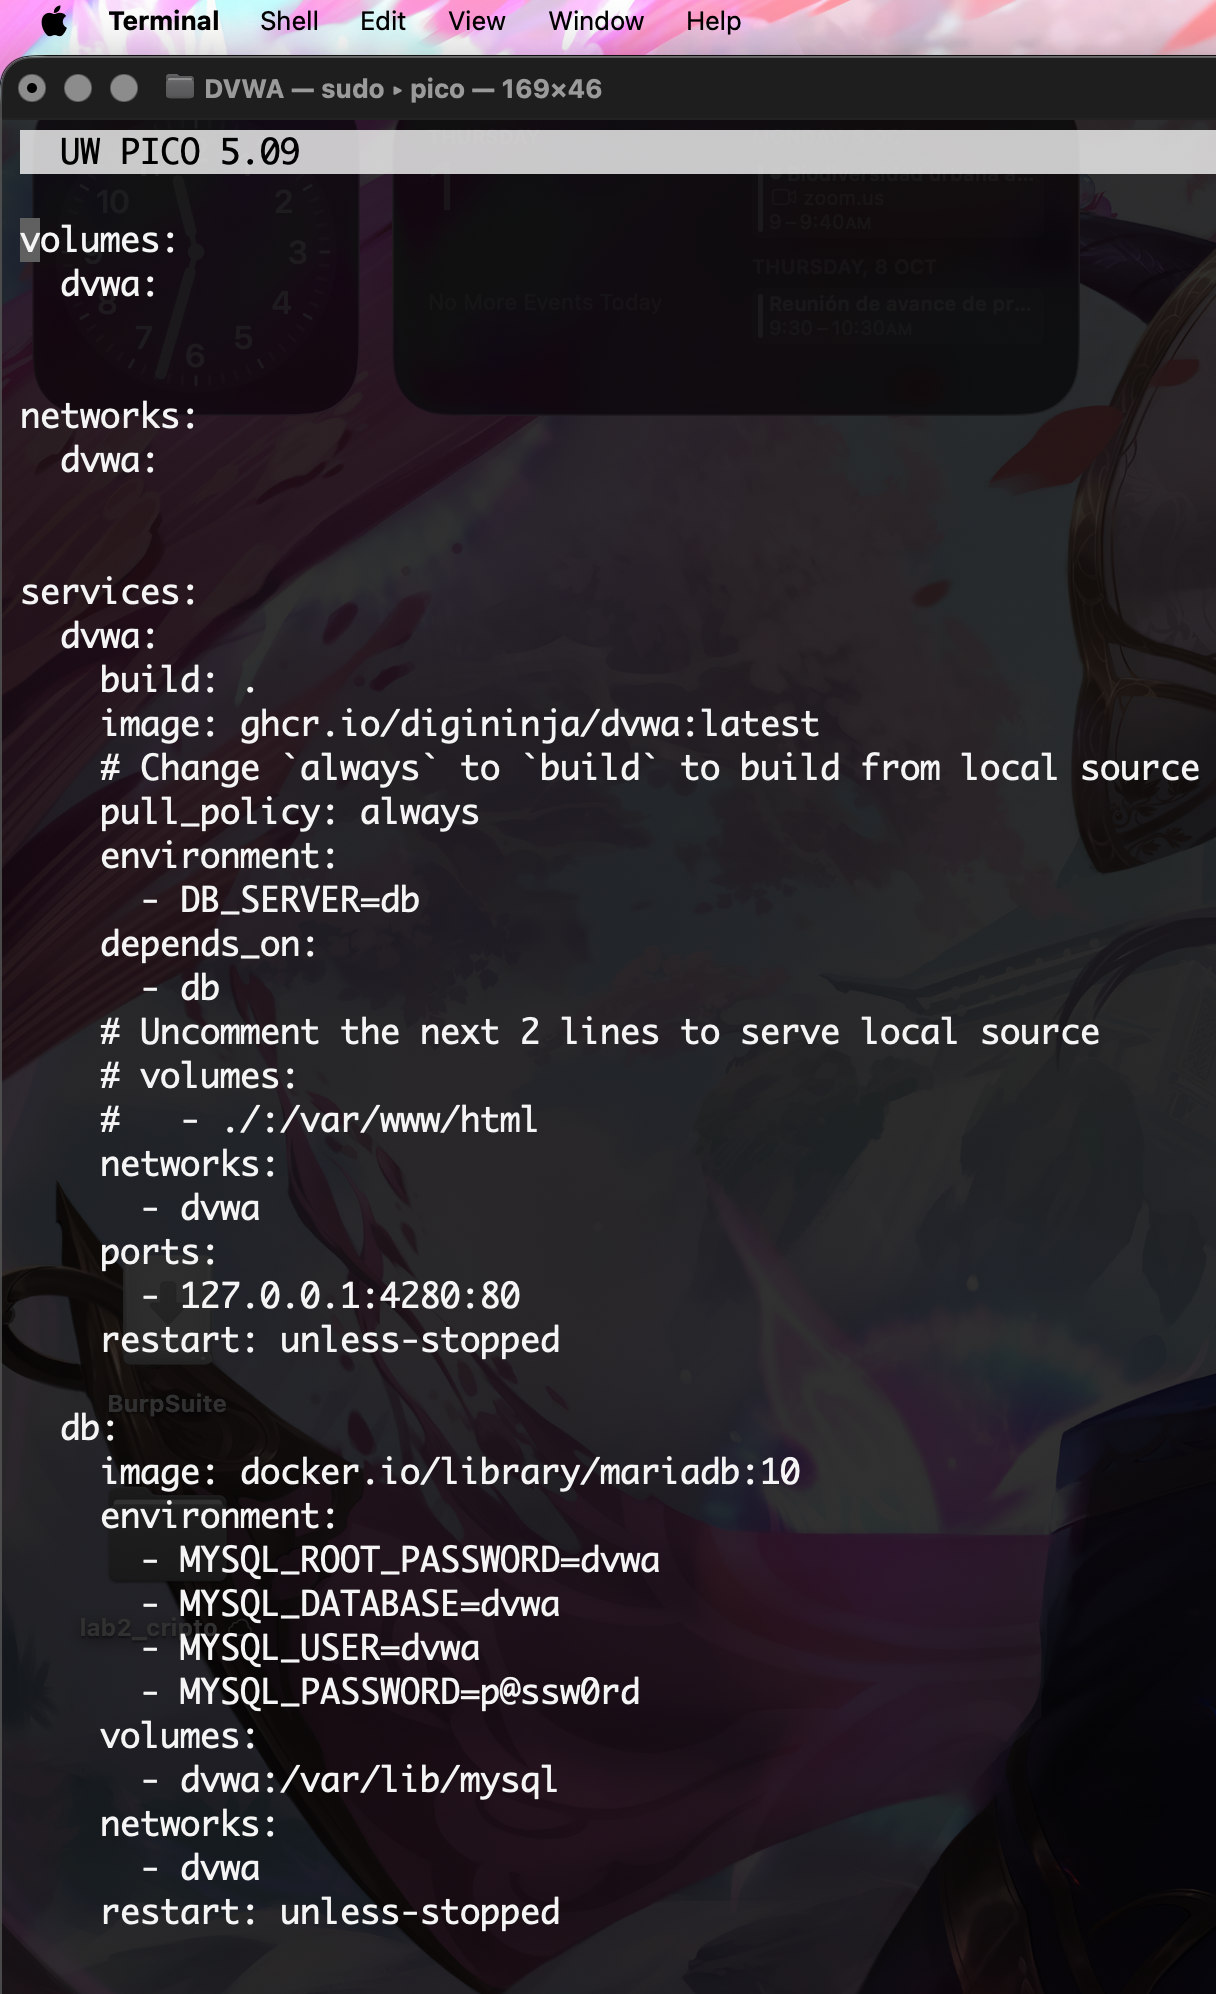
\includegraphics[width=\linewidth,height=.85\textheight,keepaspectratio]{docker_compose.jpg}
\caption{Configuración de servicios, volumen y redirección de puertos en compose.yml.}
\label{fig:dockercompose}
\end{figure}
\clearpage
\subsection{Obtención de consulta a replicar (burp)}
Se utilizó el navegador integrado de Burp Suite para ingresar a DVWA y enviar un intento desde el formulario Brute Force. Mediante Proxy se capturó una petición GET que contiene los campos \texttt{username}, \texttt{password} y \texttt{Login}. La Figura~\ref{fig:peticion} muestra la consulta interceptada.
\evidencia{burp_peticion.jpg}{Petición GET capturada mediante el proxy de Burp Suite.}{fig:peticion}
Además de los parámetros, se conservó la cabecera Cookie. El valor \texttt{PHPSESSID} mantiene la sesión de acceso a DVWA y \texttt{security=low} selecciona el nivel de seguridad utilizado. Esta sesión es independiente de las credenciales que se prueban en el formulario vulnerable.
\subsection{Identificación de campos a modificar (burp)}
La petición se envió a Intruder y se marcaron únicamente los valores de usuario y contraseña como posiciones de payload. Se seleccionó \textit{Cluster bomb}, que combina cada entrada del primer diccionario con las del segundo. El parámetro \texttt{Login=Login} se mantuvo constante.
\evidencia{burp_posiciones.jpg}{Configuración de Cluster bomb y posiciones de usuario y contraseña.}{fig:posiciones}
\subsection{Obtención de diccionarios para el ataque (burp)}
Se prepararon dos archivos de texto locales, con una entrada por línea: \texttt{usuarios.txt} y \texttt{passwords.txt}. Se utilizaron listas pequeñas para observar los resultados del laboratorio. No se descargó un diccionario masivo; las listas fueron preparadas con apoyo del asistente y cargadas como \textit{Simple list} mediante la opción Load.
\begin{lstlisting}
# usuarios.txt
admin
gordonb
1337
pablo
smithy
root
user
test
guest
administrator
# passwords.txt
password
abc123
charley
letmein
123456
admin
qwerty
welcome
test
sopas
\end{lstlisting}
Las líneas que comienzan con \texttt{\#} en el bloque anterior son títulos explicativos y no forman parte de los archivos. Con diez usuarios y diez contraseñas se definieron 100 combinaciones posibles.
\evidencia{usuarios.jpg}{Carga del diccionario de usuarios en la primera posición.}{fig:usuarios}
\evidencia{passwords.jpg}{Carga del diccionario de contraseñas en la segunda posición.}{fig:passwords}

\subsubsection*{Exploración del directorio de imágenes y selección de usuarios}
Luego de obtener un acceso válido con admin, se abrió la imagen mostrada por el formulario en otra ventana del navegador. La dirección de esa imagen era \url{http://127.0.0.1:4280/hackable/users/admin.jpg}. Al eliminar el nombre del archivo \texttt{admin.jpg} y conservar la ruta \texttt{/hackable/users/}, se intentó acceder al directorio que contenía las imágenes de los usuarios.

Inicialmente, el servidor respondió con \textit{403 Forbidden}. Al revisar los registros de Apache, se observó que no existía un archivo de índice y que el listado automático del directorio estaba deshabilitado mediante la configuración de Options. Esto explicaba que fuera posible abrir una imagen individual, pero no visualizar el contenido de la carpeta.

Como se tenía acceso administrativo al contenedor del laboratorio, se creó el archivo \texttt{lab-users-listing.conf} dentro de \texttt{/etc/apache2/conf-available/}, con la siguiente configuración:
\begin{lstlisting}
<Directory /var/www/html/hackable/users>
    Options +Indexes
</Directory>
\end{lstlisting}
Luego se habilitó la configuración, se comprobó su sintaxis y se recargó Apache:
\begin{lstlisting}
docker compose exec dvwa a2enconf lab-users-listing
docker compose exec dvwa apache2ctl configtest
docker compose exec dvwa apache2ctl graceful
\end{lstlisting}
La comprobación devolvió \texttt{Syntax OK}. Al recargar la URL en el navegador, se mostró el listado de la Figura~\ref{fig:listadousuarios}. Este procedimiento habilitó una función del servidor mediante su configuración; no correspondió a un bypass remoto del error 403.

\evidencia{listado.jpg}{Listado de /hackable/users/ luego de habilitar Options +Indexes en Apache.}{fig:listadousuarios}

En el listado se observaron los archivos \texttt{1337.jpg}, \texttt{admin.jpg}, \texttt{gordonb.jpg}, \texttt{pablo.jpg} y \texttt{smithy.jpg}. Al quitar la extensión se obtienen cinco nombres candidatos que pueden utilizarse para acotar el diccionario de usuarios. La existencia de estas imágenes no confirma por sí sola las cuentas o sus contraseñas; esa relación se comprueba mediante las respuestas del formulario.

Esta observación permite proponer una mejora al ataque: utilizar solamente esos cinco candidatos y combinarlos con las diez contraseñas del diccionario. De esta manera se pasa de 100 a 50 combinaciones posibles, reduciendo el espacio de búsqueda a la mitad. Las ejecuciones documentadas en este informe utilizaron la lista original de diez usuarios; el listado se incorpora como evidencia adicional que respalda la selección de candidatos para una prueba posterior más acotada.

\subsection{Obtención de al menos 2 pares (burp)}
Se identificaron los pares \texttt{admin/password} y \texttt{gordonb/abc123}. La validación se realizó revisando el contenido de la respuesta: los accesos correctos muestran el mensaje \textit{Welcome to the password protected area}, seguido del usuario, y una imagen asociada a este.
\evidencia{burp_admin.jpg}{Respuesta de éxito para el usuario admin.}{fig:burpadmin}
\evidencia{burp_gordon.jpg}{Credenciales gordonb/abc123 y mensaje de éxito en Burp Intruder.}{fig:burpgordon}
En cambio, un intento incorrecto muestra \textit{Username and/or password incorrect.}, como se observa en la Figura~\ref{fig:burperror}. Tanto un acceso válido como uno inválido pueden devolver HTTP 200, por lo que este código no permite confirmar el éxito por sí solo. La longitud de la respuesta ayuda a seleccionar candidatos, pero debe verificarse el mensaje recibido.
\evidencia{burp_error.jpg}{Respuesta del formulario frente a credenciales incorrectas.}{fig:burperror}
Durante una repetición del ataque se recibieron respuestas HTTP 302 con destino a \texttt{../../login.php}. Esto correspondía a una sesión no válida para acceder a DVWA, no a un resultado del formulario. Se volvió a iniciar sesión y se capturó una petición nueva con la cookie actual antes de repetir la prueba.
\subsection{Obtención de código de inspect element (curl)}
Se abrió la pestaña Network de las herramientas de desarrollador de Firefox y se realizó un acceso válido en Brute Force. Sobre la petición del formulario se seleccionó \textit{Copy as cURL}, obteniendo la URL y las cabeceras necesarias para replicarla desde Terminal.
\evidencia{curl_copy.jpg}{Obtención del comando mediante Copy as cURL en Firefox.}{fig:copy}
\subsection{Utilización de curl por terminal (curl)}
El comando copiado se ejecutó conservando las cabeceras del navegador y la cookie de sesión. Se añadió \texttt{-D} para guardar las cabeceras, \texttt{-o} para guardar el HTML y \texttt{-w} para mostrar el código HTTP. La opción \texttt{--compressed} permite solicitar una respuesta comprimida y descomprimirla al guardarla. Se dejó que cURL seleccionara las codificaciones que soporta, sin fijar manualmente Accept-Encoding.
El siguiente bloque reproduce la estructura del comando utilizado. El identificador de sesión se representa como \texttt{SESION\_ACTUAL}; en la ejecución se utilizó el valor real copiado del navegador.
\begin{lstlisting}
curl 'http://127.0.0.1:4280/vulnerabilities/brute/?username=admin&password=password&Login=Login' \
 --compressed \
 -H 'User-Agent: Mozilla/5.0 (Macintosh; Intel Mac OS X 10.15; rv:155.0) Gecko/20100101 Firefox/155.0' \
 -H 'Accept: text/html,application/xhtml+xml,application/xml;q=0.9,*/*;q=0.8' \
 -H 'Accept-Language: en-US,en;q=0.9' \
 -H 'Connection: keep-alive' \
 -H 'Referer: http://127.0.0.1:4280/vulnerabilities/brute/?username=admin&password=sopas&Login=Login' \
 -H 'Cookie: security=low; PHPSESSID=SESION_ACTUAL' \
 -H 'Upgrade-Insecure-Requests: 1' \
 -H 'Sec-Fetch-Dest: document' \
 -H 'Sec-Fetch-Mode: navigate' \
 -H 'Sec-Fetch-Site: same-origin' \
 -H 'Sec-Fetch-User: ?1' \
 -H 'DNT: 1' -H 'Sec-GPC: 1' \
 -H 'Priority: u=0, i' \
 -D valido.headers -o valido.html \
 -w '\nHTTP: %{http_code}\n'
\end{lstlisting}
Luego se repitió el comando cambiando solamente la contraseña de la URL a \texttt{incorrecta123} y los archivos de salida a \texttt{invalido.headers} e \texttt{invalido.html}. El valor \texttt{sopas} del Referer corresponde a la página de procedencia conservada en la petición, no a la contraseña probada en la URL actual.
\evidencia{curl_valido.jpg}{Ejecución de cURL con credenciales válidas y respuesta HTTP 200.}{fig:curlvalido}
\evidencia{curl_invalido.jpg}{Ejecución de cURL con contraseña incorrecta, también con HTTP 200.}{fig:curlinvalido}
\subsection{Demuestra 5 diferencias (curl)}
Para comparar las respuestas se utilizaron los siguientes comandos:
\begin{lstlisting}
diff -u invalido.html valido.html
wc -c valido.html invalido.html
\end{lstlisting}
\evidencia{curl_diff.jpg}{Comparación del HTML y medición del tamaño de ambos archivos.}{fig:diff}
La pauta solicita cuatro diferencias entre las páginas, mientras que el título de la plantilla solicita cinco. Se documentan cuatro diferencias del HTML y una medición adicional de la transferencia, distinguiendo ambos tipos de resultado.
\begin{enumerate}
\item \textbf{Mensaje:} el acceso válido devuelve la bienvenida a admin; el inválido indica que el usuario o la contraseña son incorrectos.
\item \textbf{Estructura HTML:} el mensaje válido está dentro de una etiqueta \texttt{<p>}; el error utiliza \texttt{<pre>} y un salto \texttt{<br />}.
\item \textbf{Imagen del usuario:} la respuesta válida incluye \texttt{<img>} con la ruta \texttt{/hackable/users/admin.jpg}; la inválida no incluye esa imagen.
\item \textbf{Tamaño del documento:} el HTML válido ocupa 4547 bytes y el inválido 4509 bytes, con una diferencia de 38 bytes.
\item \textbf{Bytes recibidos en la transferencia:} el indicador de cURL muestra 1469 bytes para el acceso válido y 1448 para el inválido, una diferencia de 21 bytes. Esta medición corresponde a la transferencia comprimida de estas ejecuciones, no al tamaño del HTML descomprimido medido con wc.
\end{enumerate}
Los dos intentos devolvieron HTTP 200. Por lo tanto, se confirmó el resultado mediante el cuerpo de la respuesta y no únicamente mediante el estado HTTP.
\subsection{Instalación y versión a utilizar (hydra)}
Para instalar Hydra en macOS se utilizó Homebrew. El procedimiento de instalación y la consulta de ayuda son los siguientes:
\begin{lstlisting}
brew install hydra
hydra -h
\end{lstlisting}
La versión utilizada fue Hydra 9.7, como se observa en la Figura~\ref{fig:version}. Esta captura acredita la versión disponible; no muestra el proceso de instalación.
\evidencia{hydra_version.jpg}{Versión de Hydra utilizada en el laboratorio.}{fig:version}
\subsection{Explicación de comando a utilizar (hydra)}
Se reutilizaron los diccionarios cargados en Burp y la estructura GET del formulario. El comando utilizado fue el siguiente, sustituyendo \texttt{SESION\_ACTUAL} por la cookie vigente:
\begin{lstlisting}
hydra -L usuarios.txt -P passwords.txt \
 -s 4280 -t 1 -V -o resultados_hydra.txt \
 127.0.0.1 http-get-form \
 '/vulnerabilities/brute/:username=^USER^&password=^PASS^&Login=Login:H=Cookie\: security=low; PHPSESSID=SESION_ACTUAL:S=Welcome to the password protected area'
\end{lstlisting}
\begin{itemize}
\item \texttt{-L} y \texttt{-P}: indican los archivos de usuarios y contraseñas.
\item \texttt{-s 4280}: selecciona el puerto publicado por Docker.
\item \texttt{-t 1}: utiliza una tarea de ataque a la vez.
\item \texttt{-V}: muestra las combinaciones probadas por Terminal.
\item \texttt{-o}: guarda los pares encontrados en un archivo.
\item \texttt{http-get-form}: utiliza un formulario con parámetros GET.
\item \texttt{\^{}USER\^{}} y \texttt{\^{}PASS\^{}}: se reemplazan por los valores de los diccionarios.
\item \texttt{H=Cookie}: envía la sesión y el nivel low; el carácter de dos puntos de la cabecera se escapa con una barra invertida.
\item \texttt{S=Welcome to the password protected area}: define el texto que debe aparecer para considerar válido un intento.
\end{itemize}
No se utilizó \texttt{-f}, ya que se requería obtener más de un par. Se definieron 100 combinaciones posibles, pero la salida muestra que Hydra omitió las contraseñas restantes de un usuario una vez encontrada una válida. Por ello, no se interpreta ese total como 100 solicitudes de autenticación efectivamente realizadas.
\subsection{Obtención de al menos 2 pares (hydra)}
La ejecución reportó cinco pares válidos:
\begin{center}
\begin{tabular}{ll}\hline
Usuario & Contraseña\\\hline
admin & password\\
gordonb & abc123\\
1337 & charley\\
pablo & letmein\\
smithy & password\\\hline
\end{tabular}
\end{center}
\evidencia{hydra_resultados.jpg}{Pares válidos guardados en resultados\_hydra.txt.}{fig:hydraresultados}
Para comprobar los resultados se ingresaron manualmente los pares \texttt{gordonb/abc123} y \texttt{1337/charley} en Brute Force, manteniendo la sesión de DVWA. En ambos casos se obtuvo la bienvenida correspondiente.
\evidencia{hydra_gordon.jpg}{Validación manual del usuario gordonb.}{fig:validagordon}
\evidencia{hydra_1337.jpg}{Validación manual del usuario 1337.}{fig:valida1337}
\subsection{Explicación paquete curl (tráfico)}
Se utilizó Wireshark para capturar las ejecuciones por separado en la interfaz \texttt{lo0}, con el filtro de captura \texttt{tcp port 4280}. Para seleccionar las peticiones se aplicó el filtro de visualización \texttt{http.request \&\& tcp.port == 4280}.
La petición de cURL utiliza GET y HTTP/1.1, con origen y destino local. En la captura inicial el puerto origen fue 56306 y el destino 4280. El paquete capturado ocupó 755 bytes, de los cuales 699 corresponden a datos TCP. Estas cantidades no representan el tamaño de la respuesta HTML.
\evidencia{trafico_curl.jpg}{Cabeceras de la petición generada mediante cURL.}{fig:traficocurl}
Se observan Host, Cookie, Accept, Accept-Language, Referer y las cabeceras copiadas de Firefox. Accept-Encoding anuncia deflate y gzip. El User-Agent indica Firefox porque fue definido explícitamente en el comando. Las credenciales y la cookie se observan en texto claro debido al uso de HTTP sin cifrado.
\subsection{Explicación paquete burp (tráfico)}
La petición de Burp utiliza GET y HTTP/1.1 para enviar el mismo par admin/password. Conserva las cabeceras de Chromium de la petición original, incluyendo \texttt{sec-ch-ua}, \texttt{sec-ch-ua-mobile} y \texttt{sec-ch-ua-platform}. El Referer corresponde a la ruta del formulario y Accept-Encoding anuncia gzip, deflate y br.
\evidencia{trafico_burp.jpg}{Petición enviada por Burp conservando cabeceras del navegador Chromium.}{fig:traficoburp}
La cookie PHPSESSID de esta captura es distinta a la utilizada en cURL. Esto indica una sesión diferente, no una característica propia de Burp. Durante Intruder se observó una secuencia de peticiones que modifican los parámetros de usuario y contraseña.
\subsection{Explicación paquete hydra (tráfico)}
La petición de Hydra utiliza GET y HTTP/1.0. Se observan las cabeceras Cookie, Host y User-Agent, sin las cabeceras adicionales de navegación presentes en las otras dos capturas. El User-Agent contiene \texttt{Mozilla/5.0 (Hydra)}.
\evidencia{trafico_hydra.jpg}{Petición HTTP/1.0 de Hydra con identificación explícita en User-Agent.}{fig:traficohydra}
Los datos TCP de este segmento ocupan 207 bytes. La petición es más pequeña que la de cURL porque contiene menos cabeceras y una menor longitud total. También envía las credenciales en la URL y mantiene la sesión mediante PHPSESSID.
\subsection{Mención de las diferencias (tráfico)}
\begin{table}[H]\centering\small
\begin{tabularx}{\linewidth}{|>{\raggedright\arraybackslash}p{2.7cm}|X|X|X|}\hline
Característica & cURL & Burp & Hydra\\\hline
Versión HTTP & 1.1 & 1.1 & 1.0\\\hline
User-Agent & Firefox copiado & Navegador Chromium & Mozilla/5.0 (Hydra)\\\hline
Accept-Encoding & deflate, gzip & gzip, deflate, br & Ausente\\\hline
Referer & Formulario con parámetros previos & Ruta del formulario & Ausente\\\hline
Sec-Fetch & Presente & Presente & Ausente\\\hline
Patrón utilizado & Ejecución individual & Combinaciones mediante Intruder & Intentos automatizados con diccionarios\\\hline
\end{tabularx}
\caption{Diferencias observadas en las ejecuciones del laboratorio.}
\end{table}
Estas diferencias corresponden a la configuración usada en las pruebas y no a propiedades invariables de cada programa. Los tres casos comparten el método GET, el destino local, la ruta del formulario y el uso de cookies.
\subsection{Detección de SW (tráfico)}
En la captura de Hydra se encuentra una identificación explícita en User-Agent. Sin embargo, este campo puede modificarse, por lo que no constituye una prueba definitiva del programa utilizado. Esto se evidencia con cURL, que envió un User-Agent de Firefox al replicar el comando copiado del navegador.
En Burp se conservaron cabeceras de Chromium. Su presencia permite describir la petición original, pero no demuestra por sí sola que el tráfico provenga de Intruder. La repetición de intentos con distintos pares permite reconocer un patrón de automatización, aunque ese patrón también puede producirse con otras herramientas.
Por lo tanto, para identificar software resulta necesario combinar cabeceras, versión HTTP, frecuencia y secuencia de solicitudes. En este laboratorio se conoce el origen porque se ejecutó cada herramienta por separado; un observador externo solamente dispondría de indicios.
\section*{Conclusiones y comentarios}
\addcontentsline{toc}{section}{Conclusiones y comentarios}
El laboratorio permitió comparar tres formas de interactuar con el mismo formulario: la modificación de peticiones mediante Burp, su reproducción desde Terminal con cURL y la automatización con Hydra. Se obtuvieron pares válidos con Burp y cinco pares con Hydra, verificando el resultado mediante los mensajes de bienvenida y pruebas manuales.
Una de las principales observaciones fue que HTTP 200 no indica necesariamente un acceso válido. Tanto el intento correcto como el incorrecto devolvieron ese estado, por lo que se revisó el contenido del HTML. Asimismo, una cookie no vigente provocó redirecciones al login y obligó a capturar una sesión nueva antes de continuar con Intruder.
La comparación de tráfico mostró que las herramientas pueden enviar cabeceras similares y que el User-Agent puede ser copiado o modificado. Esto limita la identificación basada en un único campo. También se comprobó que, al utilizar HTTP, las credenciales y cookies quedan visibles en las capturas.
Como actividad adicional, se revisó el error 403 de la carpeta \texttt{/hackable/users/}. El servidor tenía deshabilitado el listado automático y se habilitó mediante \texttt{Options +Indexes}. Este procedimiento fue un cambio de configuración administrativa y no un bypass de autenticación. El listado muestra nombres de archivos y no acredita, por sí solo, la existencia de cuentas válidas.
\section*{Referencias}
\addcontentsline{toc}{section}{Referencias}
\begin{itemize}
\item DVWA, repositorio y configuración Docker: \url{https://github.com/digininja/DVWA}.
\item Burp Suite Community Edition: \url{https://portswigger.net/burp/communitydownload}.
\item Hydra, fórmula de Homebrew: \url{https://formulae.brew.sh/formula/hydra}.
\item Ayuda local de Hydra 9.7: \texttt{hydra -h} y \texttt{hydra -U http-get-form}.
\item Wireshark, seguimiento de flujos: \url{https://www.wireshark.org/docs/wsug_html_chunked/ChAdvFollowStreamSection.html}.
\end{itemize}
\end{document}
